\documentclass[tikz,border=8pt]{standalone}
% Shared look for every TikZ diagram. Load with \input{../../tools/tikz-style.tex}
\usepackage[T1]{fontenc}
\usepackage{lmodern}
\renewcommand{\sfdefault}{lmr}  % diagrams use the same serif as the text
\usetikzlibrary{arrows.meta, positioning, shapes.geometric, calc, fit, backgrounds}
\definecolor{cblue}{HTML}{4C78A8}
\definecolor{corange}{HTML}{F58518}
\definecolor{cgreen}{HTML}{54A24B}
\definecolor{cred}{HTML}{E45756}
\definecolor{cpurple}{HTML}{B279A2}
\definecolor{cgrey}{HTML}{6B6B6B}
\tikzset{
  every picture/.style={font=\sffamily, line width=1.2pt},
  box/.style={draw=#1, fill=#1!12, rounded corners=4pt, align=center, inner sep=7pt, minimum height=1.1cm},
  box/.default=cgrey,
  arrow/.style={-{Stealth[length=3mm]}, draw=cgrey, line width=1.4pt},
  title/.style={font=\sffamily\bfseries\Large},
  note/.style={font=\sffamily\small, text=cgrey, align=center},
}
\AtBeginDocument{\hyphenpenalty=10000 \exhyphenpenalty=10000}

\begin{document}
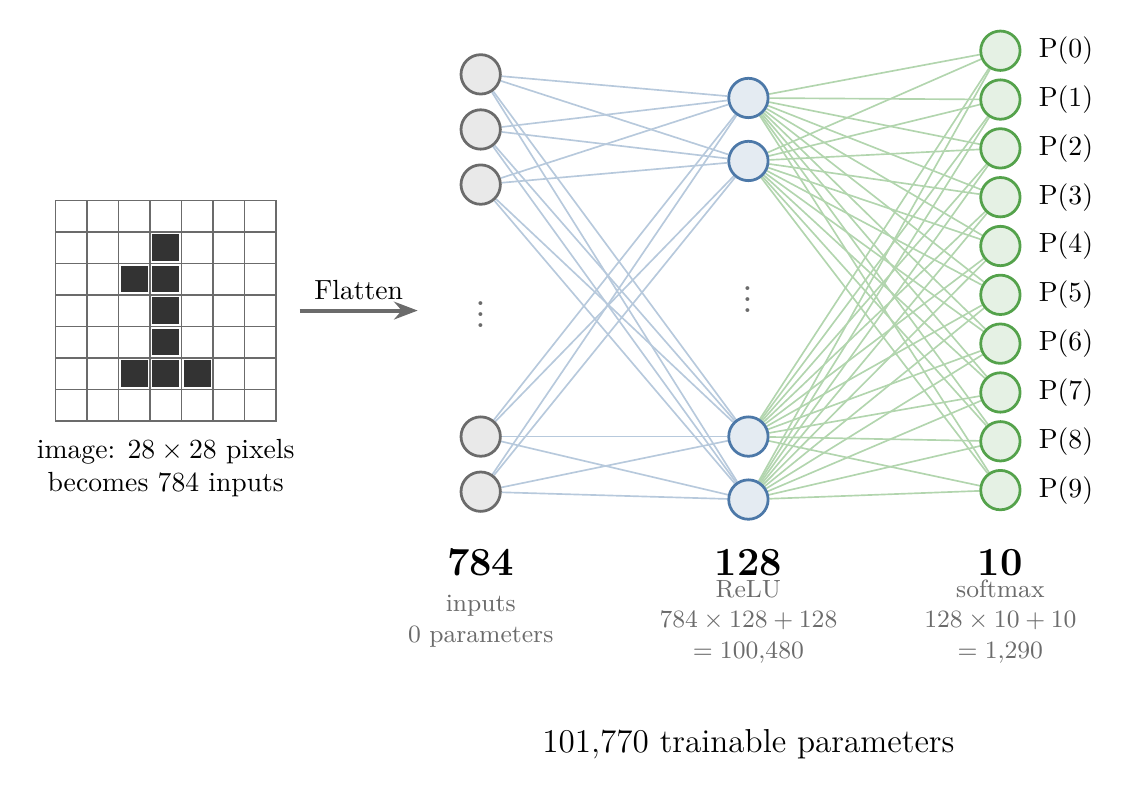
\begin{tikzpicture}[
  nd/.style={circle, draw=#1, fill=#1!15, minimum size=0.5cm, inner sep=0pt, line width=1pt},
  dots/.style={font=\sffamily\Large, text=cgrey}]
  % 28 x 28 image as a grid (drawn 7 x 7 for readability)
  \foreach \r in {0,...,6} \foreach \c in {0,...,6}
    \draw[cgrey, line width=0.5pt, fill=white] (\c*0.4, -\r*0.4) rectangle ++(0.4,-0.4);
  \foreach \r/\c in {1/3,2/2,2/3,3/3,4/3,5/2,5/3,5/4}
    \fill[black!80] (\c*0.4+0.03, -\r*0.4-0.03) rectangle ++(0.34,-0.34);
  \node[font=\sffamily\normalsize, align=center] at (1.4, -3.4) {image: $28 \times 28$ pixels\\becomes 784 inputs};
  % Flatten
  \draw[arrow] (3.1, -1.4) -- node[above, font=\sffamily\normalsize] {Flatten} (4.6, -1.4);
  % input layer: 784 nodes
  \foreach \i/\y in {1/1.6, 2/0.9, 3/0.2, 4/-3.0, 5/-3.7} \node[nd=cgrey] (x\i) at (5.4, \y) {};
  \node[dots] at (5.4, -1.35) {$\vdots$};
  % hidden layer: 128 nodes
  \foreach \j/\y in {1/1.3, 2/0.5, 3/-3.0, 4/-3.8} \node[nd=cblue] (h\j) at (8.8, \y) {};
  \node[dots] at (8.8, -1.15) {$\vdots$};
  % output layer: 10 nodes, one per digit
  \foreach \k in {0,...,9} {
    \node[nd=cgreen] (o\k) at (12.0, 1.9-0.62*\k) {};
    \node[font=\sffamily\normalsize, anchor=west] at (12.35, 1.9-0.62*\k) {P(\k)};
  }
  \begin{scope}[on background layer]
    \foreach \i in {1,...,5} \foreach \j in {1,...,4} \draw[cblue!40, line width=0.6pt] (x\i) -- (h\j);
    \foreach \j in {1,...,4} \foreach \k in {0,...,9} \draw[cgreen!45, line width=0.6pt] (h\j) -- (o\k);
  \end{scope}
  % labels under the layers
  \node[title] at (5.4, -4.6) {784};
  \node[note] at (5.4, -5.35) {inputs\\0 parameters};
  \node[title] at (8.8, -4.6) {128};
  \node[note] at (8.8, -5.35) {ReLU\\$784 \times 128 + 128$\\$= 100{,}480$};
  \node[title] at (12.0, -4.6) {10};
  \node[note] at (12.0, -5.35) {softmax\\$128 \times 10 + 10$\\$= 1{,}290$};
  \node[font=\sffamily\large] at (8.8, -6.9) {101,770 trainable parameters};
\end{tikzpicture}
\end{document}
